\documentclass[journal,twoside]{IEEEtran}

\usepackage{cite}
\usepackage{amsmath,amssymb,amsfonts}
\usepackage{algorithm}
\usepackage{algpseudocode}
\usepackage{graphicx}
\usepackage{textcomp}
\usepackage{xcolor}
\usepackage{hyperref}
\usepackage{booktabs}
\usepackage{subcaption}
\usepackage{bm}
\usepackage{tikz}
\usetikzlibrary{arrows.meta, positioning, calc, fit, backgrounds}

\begin{document}

\title{Decoupled Reactive Safety Filtering for Generative Trajectory Policies via Bernstein Robot Distance Fields and Control Barrier Functions}

\author{Fr\'ed\'erick Lanthier, Sofiane Achiche, and J\'er\^ome Le Ny
\thanks{This work was supported by Polytechnique Montr\'eal.}
\thanks{Fr\'ed\'erick Lanthier, Sofiane Achiche, and J\'er\^ome Le Ny are with the Department of Mechanical Engineering, Polytechnique Montr\'eal, QC H3T 1J4, Canada (e-mail: frederick.lanthier@polymtl.ca).}
}

\markboth{IEEE Robotics and Automation Letters}{Lanthier \MakeLowercase{\textit{et al.}}: Decoupled Reactive Safety Filtering for Generative Trajectory Policies}

\maketitle

\begin{abstract}
Generative trajectory policies based on Flow Matching (FM) exhibit strong performance in capturing multimodal expert demonstrations for robotic manipulation. However, when trained on obstacle-free demonstrations, they lack formal safety guarantees in unseen, cluttered environments. Retraining or constraining the generative sampling process introduces severe computational overhead and distributional shift. In this paper, we propose a fully decoupled architecture that decouples trajectory intent from real-time safety enforcement. A frozen, pre-trained FM policy generates nominal joint trajectories, while a downstream reactive Control Barrier Function (CBF) shield filters velocity commands at 100~Hz. To enable high-frequency, whole-body obstacle avoidance, we construct a Robot Distance Field (RDF) using 3D Bernstein polynomials refined via a two-stage training scheme that explicitly constrains distance values, Eikonal gradient norms, and surface-normal directional alignment on 20,000 verified rays. We derive an exact, closed-form analytical expression for the joint-space distance gradient using link geometric Jacobians, avoiding auto-differentiation overhead. The CBF formulation incorporates a three-layer tightening scheme covering discretization, low-level tracking error, and moving obstacles, supplemented by a 1~kHz C++ reflex brake. Validated in simulation on 7-DoF Franka Emika Panda and UFactory xArm7 manipulators for assisted feeding and pick-and-place tasks, our framework completely eliminates collisions without degrading task success, while maintaining sub-millisecond QP execution times and zero-shot transfer across robot embodiments.
\end{abstract}

\begin{IEEEkeywords}
Reactive safety filtering, Flow Matching, Control Barrier Functions, Robot Distance Fields, robotic manipulation.
\end{IEEEkeywords}

\section{Introduction}
\IEEEPARstart{G}{enerative} behavior cloning models, notably Diffusion Policies \cite{ChiXXXXVisuomotor, Ho2020Denoising, Janner2022Planning} and Flow Matching (FM) \cite{Lipman2023Flow, Tong2024Conditional, Liu2023Rectified}, have emerged as powerful frameworks for robotic manipulation. By learning continuous velocity vector fields from expert demonstrations, FM planners generate smooth, multimodal trajectories in a small number of deterministic integration steps, enabling closed-loop replanning. 

Despite these advances, generative policies remain fundamentally constrained by their training data: when trained on obstacle-free demonstrations, they offer no safety guarantees when deployed in unobserved, cluttered environments. Traditional motion planners (e.g., RRT-Connect \cite{Kuffner2000Rrt}, OMPL \cite{Sucan2012Ompl}, CHOMP \cite{Zucker2013Chomp}, TrajOpt \cite{Schulman2014Trajopt}) can navigate around obstacles but lack the rich task multimodal priors captured by generative networks. Existing attempts to address safety in generative planners fall into two main paradigms, both carrying substantial drawbacks:
\begin{enumerate}
    \item \textit{Generative Constraining:} Modifying the sampling process itself via guided diffusion \cite{Dai2025Safeflow, Yang2026Safeflowmatcher} or constrained ODE integration causes distributional shift and incurs heavy computational latency at every sampling iteration.
    \item \textit{Obstacle-Aware Retraining:} Teaching avoidance to the generative model requires massive dataset augmentation with cluttered scenes or human-in-the-loop corrections \cite{Welte2026Flowcorrect}, requiring retraining for every scene geometry.
\end{enumerate}

To overcome these limitations, we propose a third paradigm: \textit{filtering execution rather than generation} \cite{Rmer2026From, Wabersich2021Predictive}. As illustrated in Fig.~\ref{fig:architecture}, our framework completely decouples nominal task intention from safety enforcement. A pre-trained, frozen FM policy generates nominal joint trajectories at 3--5~Hz. Downstream of the model, a reactive Control Barrier Function (CBF) filter \cite{Ames2019Control, Ames2017Control} evaluates whole-body safety against a persistent scene map and projects velocity commands at 100~Hz to enforce prospective invariance of the safe set.

\begin{figure}[t]
    \centering
    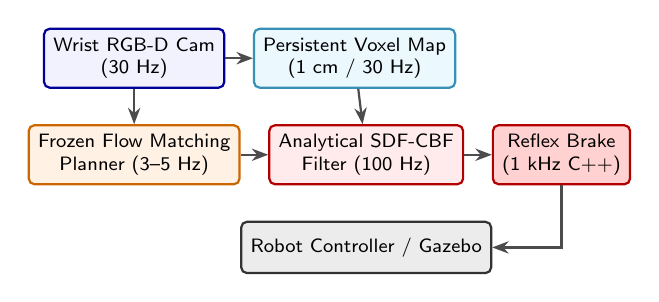
\begin{tikzpicture}[
        font=\sffamily\scriptsize,
        node distance=0.45cm and 0.35cm,
        box/.style={draw, rounded corners=2pt, thick, align=center, minimum height=0.65cm, fill=blue!5, draw=blue!60!black},
        safe/.style={box, fill=red!8, draw=red!70!black},
        map/.style={box, fill=cyan!8, draw=cyan!70!black},
        gen/.style={box, fill=orange!10, draw=orange!80!black},
        arr/.style={-{Stealth[scale=0.9]}, thick, draw=black!70}
    ]
        \node[box] (cam) {Wrist RGB-D Cam\\(30 Hz)};
        \node[map, right=of cam] (map) {Persistent Voxel Map\\(1 cm / 30 Hz)};
        \node[gen, below=of cam] (fm) {Frozen Flow Matching\\Planner (3--5 Hz)};
        \node[safe, right=of fm] (cbf) {Analytical SDF-CBF\\Filter (100 Hz)};
        \node[safe, fill=red!18, right=of cbf] (rfx) {Reflex Brake\\(1 kHz C++)};
        \node[box, fill=gray!15, draw=black!80, below=of cbf] (robot) {Robot Controller / Gazebo};

        \draw[arr] (cam) -- (map);
        \draw[arr] (cam) -- (fm);
        \draw[arr] (map) -- (cbf);
        \draw[arr] (fm) -- (cbf);
        \draw[arr] (cbf) -- (rfx);
        \draw[arr] (rfx) |- (robot);
    \end{tikzpicture}
    \caption{System architecture showing the 4-tier asynchronous control pipeline: 3--5~Hz Flow Matching trajectory generator, 30~Hz persistent voxel map, 100~Hz analytical SDF-CBF safety filter, and 1~kHz C++ reflex brake.}
    \label{fig:architecture}
\end{figure}

The primary bottleneck of whole-body CBF filtering lies in obtaining accurate, continuously differentiable signed distance fields (SDFs) of all robot links and their analytical joint-space gradients at control frequencies ($>100$~Hz). Standard Robot Distance Fields (RDF) \cite{Li2024rdf, Li2024Configuration} approximate link SDFs with Bernstein polynomials via recursive least squares (RLS), but fitting distance values alone produces noisy, magnitude-distorted spatial gradients near link surfaces---precisely where CBFs require exact directionality.

In this work, we resolve this bottleneck and present the following main contributions:
\begin{itemize}
    \item A fully decoupled, training-free safety architecture combining a frozen FM policy with a whole-body reactive SDF-CBF filter and a persistent voxel map.
    \item A two-stage offline learning scheme for Bernstein RDFs combining RLS value regression with a multi-objective geometric refinement loss enforcing Eikonal gradient norms ($\|\nabla\bar{d}\|=1$) and directional alignment on 20,000 verified normal rays.
    \item An exact, closed-form analytical joint-space distance gradient derived via rigid-body geometric Jacobians \cite{Carpentier2019Pinocchio}, eliminating automatic differentiation overhead.
    \item A smooth, monotone out-of-domain minorant extension preserving physical gradient orientation outside the approximation domain.
    \item A three-layer constraint tightening scheme (addressing zero-order hold discretization, tracking error, and moving obstacles) coupled with a nested 1~kHz C++ reflex brake.
    \item Empirical validation in simulation on Franka Emika Panda and UFactory xArm7 manipulators, demonstrating zero collisions, task success preservation, and cross-embodiment transfer.
\end{itemize}

\section{Related Work}

\subsection{Generative Policies in Manipulation}
Behavior cloning via generative modeling has revolutionized robot manipulation. Diffusion policies \cite{ChiXXXXVisuomotor, Ho2020Denoising} and Flow Matching models \cite{Lipman2023Flow, Tong2024Conditional, Liu2023Rectified} capture complex multimodal action distributions. Flow Matching models straight-line vector fields, enabling deterministic sampling via fast ODE numerical integrators. However, ensuring collision avoidance in test-time environments without retraining remains an open challenge \cite{Rmer2026From, Welte2026Flowcorrect}.

\subsection{Robot Distance Fields (RDF) and Scene Mapping}
Whole-body collision avoidance requires rapid distance queries between all robot links and arbitrary environmental obstacles. While 3D mapping frameworks (e.g., Voxblox \cite{Oleynikova2017Voxblox}, nvblox \cite{Millane2024Nvblox}, iSDF \cite{Ortiz2022Isdf}) map the environment, querying distances against complex meshes is computationally demanding. Robot Distance Fields \cite{Li2024rdf, Li2024Configuration, Govoni2026rdf} model each link's SDF using 3D Bernstein tensor-product polynomials in a normalized local frame. However, standard RDFs rely on automatic differentiation (autograd) or numerical differences for joint gradients, and fitting values alone leads to degraded gradient fidelity near surfaces.

\subsection{Control Barrier Functions (CBFs) and Safety Filtering}
Control Barrier Functions \cite{Ames2019Control, Ames2017Control} provide formal guarantees of forward invariance for safe sets $\mathcal{C} = \{\mathbf{q} \mid h(\mathbf{q}) \ge 0\}$. When paired with Quadratic Programs (QP), CBFs minimally modify nominal control inputs \cite{Wabersich2021Predictive, Wabersich2023Data}. In discrete-time real-time deployment, standard CBFs suffer from discretization errors, tracking delays, and local minima, requiring specialized tightening \cite{Agrawal2017Discrete, Kolathaya2019Input} and nullspace postural clearance.

\section{System Architecture and Problem Formulation}

\subsection{Asynchronous Multi-Tier Control Pipeline}
The proposed architecture operates across four asynchronous rate tiers:
\begin{enumerate}
    \item \textbf{Perception Tier (Asynchronous / 5~Hz):} Segment Anything Model 3 (SAM 3) \cite{Meta2025Sam3} initializes target segmentation from text prompts, while SAM 2 \cite{Ravi2024Sam2} tracks target masks in 512$\times$512 RGB-D images at 5~Hz.
    \item \textbf{Mapping Tier (30~Hz):} A persistent 1~cm sparse voxel grid accumulates obstacle points, featuring free-space ray-casting eviction to remove cleared voxels within the moving wrist-camera field of view.
    \item \textbf{Generative Tier (3--5~Hz):} A 1D conditional U-Net FM policy predicts nominal joint trajectory segments $\mathbf{X} \in \mathbb{R}^{H \times 7}$ conditioned on target point clouds.
    \item \textbf{Reactive Control Shield (100~Hz / 1~kHz):} An analytical SDF-CBF filter solves a QP at 100~Hz, while a nested C++ reflex node re-certifies commands at 1~kHz within `ros\_control`.
\end{enumerate}

\subsection{Problem Statement}
Let $\mathbf{q} \in \mathbb{R}^7$ be the joint configuration of a 7-DoF manipulator. Given a nominal velocity vector $\dot{\mathbf{q}}_{\mathrm{base}}$ generated by the frozen FM policy, the objective is to find a filtered velocity command $\dot{\mathbf{q}}^\star$ that minimally deviates from $\dot{\mathbf{q}}_{\mathrm{base}}$ while guaranteeing that no point on any protected link $l \in \{1,\dots,9\}$ intersects environmental obstacles $\mathbf{p}_i \in \mathcal{P}_{\mathrm{obs}}$:
\begin{equation}
    \min_{\dot{\mathbf{q}} \in \mathbb{R}^7} \frac{1}{2} \|\dot{\mathbf{q}} - \dot{\mathbf{q}}_{\mathrm{base}}\|_{\mathbf{W}}^2 \quad \text{s.t.} \quad \nabla h_l(\mathbf{q})^\top \dot{\mathbf{q}} \ge b(h_l(\mathbf{q})), \; \forall l
\end{equation}
where $\mathbf{W} \succ 0$ is a task-weighted metric and $h_l(\mathbf{q})$ is the link barrier function.

\section{Bernstein Robot Distance Field with Geometric Refinement}

\subsection{Bernstein Tensor Polynomial SDF Representation}
Each protected robot link $l$ is centered and scaled into the normalized unit cube $[-1,1]^3$:
\begin{equation}
    \bar{\mathbf{x}} = \frac{\mathbf{x} - \mathbf{o}_l}{s_l}, \quad \mathbf{u} = \frac{\bar{\mathbf{x}} + \mathbf{1}}{2} \in [0,1]^3
\end{equation}
where $\mathbf{o}_l$ is the bounding box center and $s_l$ is the scaling factor. On $[0,1]^3$, the normalized SDF $\bar{d}_l(\bar{\mathbf{x}})$ is represented by a 3D tensor product of degree $n-1 = 11$ Bernstein polynomials ($12^3 = 1728$ weights $\mathbf{w}_l$):
\begin{equation}
    \bar{d}_l(\bar{\mathbf{x}}) = \sum_{a,b,c=0}^{n-1} w^{(l)}_{abc} B_a(u_x) B_b(u_y) B_c(u_z) = \boldsymbol{\Phi}(\bar{\mathbf{x}}) \mathbf{w}_l
\end{equation}
Metric distance is recovered via $d_l(\mathbf{x}) = s_l \bar{d}_l(\bar{\mathbf{x}})$.

\subsection{Two-Stage Offline Training \& Geometric Refinement}
Standard fitting optimizes distance values alone via Recursive Least Squares (RLS) with Ridge regularization:
\begin{equation}
    \mathcal{L}_{\mathrm{RLS}} = \mathbb{E}_{\mathbf{x}} \big[ (\bar{d}_l(\mathbf{x}) - y_{\mathrm{gt}})^2 \big] + \lambda_{\mathrm{ridge}} \|\mathbf{w}_l\|^2
\end{equation}
While RLS achieves low mean distance error, it produces noisy spatial gradients $\nabla_{\mathbf{x}} \bar{d}_l$ near surface boundaries. To resolve this, we introduce a second-stage geometric refinement fine-tuning stage using AdamW on a multi-objective loss:
\begin{equation}
    \begin{aligned}
        \mathcal{L} &= \mathcal{L}_{\mathrm{val}} + \lambda_{\mathrm{eik}} \mathbb{E}\Big[ (\|\nabla \bar{d}_l\| - 1)^2 \Big] \\
        &+ \mathbb{E}\Big[ \omega(d) \Big( \lambda_{\mathrm{dir}} (1 - \widehat{\nabla \bar{d}_l} \cdot \hat{\mathbf{n}}) + \lambda_{\mathrm{vec}} \|\nabla \bar{d}_l - \hat{\mathbf{n}}\|^2 \Big) \Big]
    \end{aligned}
\end{equation}
where supervision is provided by $20,000$ verified normal rays generated by offsetting mesh surface points along face normals by random displacements $\delta \in [0, 30~\mathrm{mm}]$ and validating non-intersection against exact CAD geometry.

\subsection{Monotone Out-of-Domain Extension}
For points outside $[-1,1]^3$, clamping to the boundary point $\mathbf{c} = \mathrm{clamp}(\bar{\mathbf{x}}, -1, 1)$ with a standard Lipschitz bound $d(\mathbf{c}) - \|\bar{\mathbf{x}} - \mathbf{c}\|$ causes gradient direction reversal. We propose a smooth, monotone lower-bounding extension:
\begin{equation}
    \hat{d}(\bar{\mathbf{x}}) = \sqrt{d(\mathbf{c})^2 + \|\bar{\mathbf{x}} - \mathbf{c}\|^2}
\end{equation}
Geometrically, for any surface point $\mathbf{s}$, $|x_j - s_j|^2 \ge |c_j - s_j|^2 + |x_j - c_j|^2$ holds along every bounded axis $j$, proving $d(\bar{\mathbf{x}})^2 \ge d(\mathbf{c})^2 + \|\bar{\mathbf{x}} - \mathbf{c}\|^2$. Thus $\hat{d}(\bar{\mathbf{x}}) \le d(\bar{\mathbf{x}})$ always holds, guaranteeing safe distance underestimation while maintaining outward-pointing gradients:
\begin{equation}
    \nabla \hat{d} = \frac{d(\mathbf{c}) \nabla d(\mathbf{c})|_{\mathrm{int}} + (\bar{\mathbf{x}} - \mathbf{c})}{\hat{d}}
\end{equation}

\section{Closed-Form Analytical SDF-CBF Reactive Shield}

\subsection{Closed-Form Analytical Joint Gradient}
For a point $\mathbf{p}_i \in \mathcal{P}_{\mathrm{obs}}$, local position $\mathbf{x}_{l,i} = (\mathbf{R}_l^b)^\top (\mathbf{p}_i - \mathbf{d}_l^b)$ satisfies $\mathbf{p}_i = \mathbf{d}_l^b + \mathbf{R}_l^b \mathbf{x}_{l,i}$. Differentiating under stationary obstacle assumption ($\dot{\mathbf{p}}_i = \mathbf{0}$):
\begin{equation}
    \mathbf{0} = \dot{\mathbf{d}}_l^b + \dot{\mathbf{R}}_l^b \mathbf{x}_{l,i} + \mathbf{R}_l^b \dot{\mathbf{x}}_{l,i}
\end{equation}
Substituting linear and angular link Jacobians $\dot{\mathbf{d}}_l^b = \mathbf{J}_{L,l}^b \dot{\mathbf{q}}$ and $\dot{\mathbf{R}}_l^b = [\mathbf{J}_{A,l}^b \dot{\mathbf{q}}]_\times \mathbf{R}_l^b$, multiplying by $(\mathbf{R}_l^b)^\top$, and applying cross-product identities yields the local position Jacobian $\mathbf{J}_{x_{l,i}} = \partial \mathbf{x}_{l,i} / \partial \mathbf{q}$:
\begin{equation}
    \mathbf{J}_{x_{l,i}}(\mathbf{q}) = -(\mathbf{R}_l^b)^\top \mathbf{J}_{L,l}^b + [\mathbf{x}_{l,i}]_\times (\mathbf{R}_l^b)^\top \mathbf{J}_{A,l}^b
\end{equation}
Chain-rule composition with spatial metric gradient $\mathbf{g}_{l,i} = \mathbf{R}_l^b \nabla_{\mathbf{x}} d_{l,i}$ yields the exact joint-space distance gradient:
\begin{equation}
    \boxed{\nabla_{\mathbf{q}} d_{l,i} = -(\mathbf{J}_{L,l}^b)^\top \mathbf{g}_{l,i} - (\mathbf{J}_{A,l}^b)^\top (\mathbf{r}_{l,i} \times \mathbf{g}_{l,i})}
\end{equation}
where $\mathbf{r}_{l,i} = \mathbf{p}_i - \mathbf{d}_l^b$. This closed-form evaluation requires only two matrix-vector products and one cross-product per obstacle point, completely avoiding automatic differentiation overhead.

\subsection{Soft-Min Aggregation and Saturated CBF}
For link $l$, point distances $d_{l,i}$ are aggregated over Top-$K$ ($K=64$) critical points using Log-Sum-Exp soft-min of temperature $\alpha$:
\begin{equation}
    h_l(\mathbf{q}) = m_l - \alpha \log \sum_{i=1}^K \exp \left( -\frac{d_{l,i} - m_l}{\alpha} \right) - d_{\mathrm{safe}}
\end{equation}
where $m_l = \min_i d_{l,i}$ and $d_{\mathrm{safe}} = 15~\mathrm{mm}$. The smooth gradient is $\nabla_{\mathbf{q}} h_l = \sum_i \omega_i \nabla_{\mathbf{q}} d_{l,i}$ with weights $\omega_i = \mathrm{softmax}_i(-d_{l,i}/\alpha)$.

\begin{figure}[t]
    \centering
    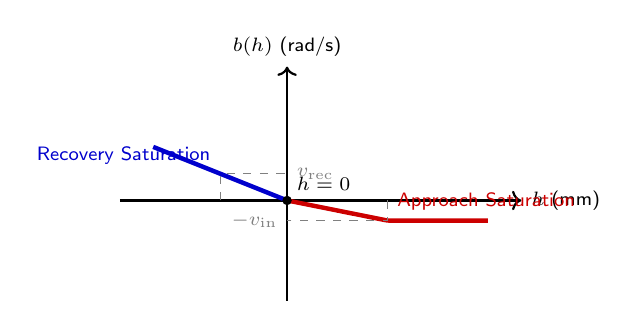
\begin{tikzpicture}[
        font=\sffamily\scriptsize,
        scale=0.85
    ]
        \draw[->, thick] (-2.5,0) -- (3.5,0) node[right] {$h$ (mm)};
        \draw[->, thick] (0,-1.5) -- (0,2.0) node[above] {$b(h)$ (rad/s)};
        
        \draw[red!80!black, ultra thick, domain=0:3, samples=100] plot (\x, {-0.3*min(\x/1.5, 1.0)});
        \draw[blue!80!black, ultra thick, domain=-2:0, samples=100] plot (\x, {-0.4*min(\x/1.0, 1.0)});
        
        \draw[dashed, gray] (1.5,0) -- (1.5,-0.3) -- (0,-0.3) node[left] {$-v_{\mathrm{in}}$};
        \draw[dashed, gray] (-1.0,0) -- (-1.0,0.4) -- (0,0.4) node[right] {$v_{\mathrm{rec}}$};
        
        \node[above right, red!80!black] at (1.5,-0.3) {Approach Saturation};
        \node[above left, blue!80!black] at (-1.0,0.4) {Recovery Saturation};
        \fill[black] (0,0) circle (2pt) node[above right] {$h=0$};
    \end{tikzpicture}
    \caption{Saturated Control Barrier Function RHS $b(h)$, showing approach velocity saturation $-v_{\mathrm{in}}$, recovery saturation $v_{\mathrm{rec}}$, and exact vanishing at the safety margin $h=0$.}
    \label{fig:saturated_cbf}
\end{figure}

The CBF constraint function $b(h)$ (illustrated in Fig.~\ref{fig:saturated_cbf}) is saturated to prevent extreme control actions:
\begin{equation}
    b(h) = \begin{cases}
        -v_{\mathrm{in}} \min(h/h_{\mathrm{act}}, 1), & h > 0 \\
        v_{\mathrm{rec}} \min(-h/d_{\mathrm{rec}}, 1), & h \le 0
    \end{cases}
\end{equation}
where $v_{\mathrm{in}} = 0.3~\mathrm{rad/s}$, $v_{\mathrm{rec}} = 0.4~\mathrm{rad/s}$, $h_{\mathrm{act}} = 80~\mathrm{mm}$, and $d_{\mathrm{rec}} = 15~\mathrm{mm}$. Restrestricted to $[-d_{\mathrm{rec}}, h_{\mathrm{act}}]$, $\gamma(h) = -b(h)$ is strictly increasing, zero at origin, and locally Lipschitz continuous, satisfying extended class-$\mathcal{K}_e$ conditions for prospective invariance.

\subsection{Three-Layer Constraint Tightening}
To bridge continuous theory and 100~Hz discrete execution:
\begin{enumerate}
    \item \textbf{Discretization Tightening:} Accounts for zero-order hold over period $T=10~\mathrm{ms}$ using Lipschitz constant $L_l$:
    \begin{equation}
        \Delta b_{\mathrm{zoh}} = \frac{1}{2} L_l T \|\dot{\mathbf{q}}\|^2
    \end{equation}
    \item \textbf{Tracking Error Tightening:} Protects against low-level execution deviation $\mathbf{d}$ bounded by $\varepsilon_{\mathrm{p}} = 0.025~\mathrm{rad/s}$:
    \begin{equation}
        \Delta b_{\mathrm{track}} = \varepsilon_{\mathrm{p}} \|\nabla h_l\|
    \end{equation}
    \item \textbf{Dynamic Obstacle Tightening:} Adjusts margin based on estimated obstacle approach velocity $\bar{d}_l$:
    \begin{equation}
        \eta_l = \mathrm{clip}(-\bar{d}_l - \varepsilon_{\mathrm{env}}, 0, \eta_{\max})
    \end{equation}
\end{enumerate}
The tightened QP constraint becomes $\nabla h_l^\top \dot{\mathbf{q}} \ge b(h_l) + \eta_l + \Delta b_{\mathrm{zoh}} + \Delta b_{\mathrm{track}}$.

\subsection{Postural Nullspace Clearance \& 1~kHz Reflex Brake}
To prevent joint-space local minima, when task progress freezes, a postural clearance velocity is projected into the Jacobian nullspace:
\begin{equation}
    \dot{\mathbf{q}}_{\mathrm{null}} = k_{\mathrm{clear}} (\mathbf{I} - \mathbf{J}^+ \mathbf{J}) \nabla h_l
\end{equation}
Finally, a nested C++ node at 1~kHz monitors executed states; if inter-sample extrapolation predicts $h \le 0$, it triggers a réflexe braking veto. Projection onto convex constraint sets is solved via Dykstra's algorithm with relaxation \cite{Dykstra1983Restricted, Boyle1986Method}, and singular kinematics are handled via damped pseudo-inversion \cite{Nakamura1986Singularity}.

\begin{algorithm}[t]
\caption{Real-Time Analytical SDF-CBF Safety Shield (100~Hz Loop)}
\label{alg:cbf_shield}
\begin{algorithmic}[1]
\Require Current joint state $\mathbf{q}$, nominal base velocity $\dot{\mathbf{q}}_{\mathrm{base}}$, obstacle point cloud $\mathcal{P}_{\mathrm{obs}}$.
\Ensure Filtered joint velocity command $\dot{\mathbf{q}}^\star$.
\State Compute forward kinematics poses $\mathbf{T}_l^b(\mathbf{q})$ for all protected links $l \in \{1,\dots,9\}$ via Pinocchio \cite{Carpentier2019Pinocchio}.
\State Extract Top-$K$ ($K=64$) critical obstacle points $\mathcal{P}_{\mathrm{CBF}} \subset \mathcal{P}_{\mathrm{obs}}$ on GPU.
\For{each protected link $l=1$ \textbf{to} $9$}
    \State Evaluate Bernstein SDF metric distances $d_{l,i}$ and spatial gradients $\mathbf{g}_{l,i}$.
    \State Compute analytical joint gradient $\nabla_{\mathbf{q}} d_{l,i} = -(\mathbf{J}_{L,l}^b)^\top \mathbf{g}_{l,i} - (\mathbf{J}_{A,l}^b)^\top (\mathbf{r}_{l,i} \times \mathbf{g}_{l,i})$.
    \State Aggregate link barrier $h_l(\mathbf{q})$ and smooth gradient $\nabla_{\mathbf{q}} h_l$ via Log-Sum-Exp.
    \State Compute saturated RHS $b(h_l)$ and tightening terms $\Delta b_{\mathrm{zoh}}, \Delta b_{\mathrm{track}}, \eta_l$.
\EndFor
\State Assemble top $K_a=9$ link constraints $\mathbf{A} \dot{\mathbf{q}} \ge \mathbf{b}_{\mathrm{tight}}$.
\State Solve QP projection $\min_{\dot{\mathbf{q}}} \frac{1}{2} \|\dot{\mathbf{q}} - \dot{\mathbf{q}}_{\mathrm{base}}\|_{\mathbf{W}}^2$ via Dykstra's algorithm \cite{Dykstra1983Restricted} with relaxation ($\omega=1.0$, $N_{\mathrm{it}}=6$).
\If{Task progress frozen}
    \State Inject postural nullspace clearance $\dot{\mathbf{q}}^\star \leftarrow \dot{\mathbf{q}}^\star + k_{\mathrm{clear}} (\mathbf{I} - \mathbf{J}^+ \mathbf{J}) \nabla h_l$.
\EndIf
\State \Return Filtered velocity command $\dot{\mathbf{q}}^\star$.
\end{algorithmic}
\end{algorithm}

\section{Experimental Evaluation and Results}

\begin{table}[t]
\caption{System Hyperparameters and Operational Constraints.}
\label{tab:hyperparams}
\centering
\begin{tabular}{lcc}
\toprule
\textbf{Parameter} & \textbf{Symbol} & \textbf{Value} \\
\midrule
Safety Margin & $d_{\mathrm{safe}}$ & $15~\mathrm{mm}$ \\
Top-$K$ Point Selection & $K$ & $64$ \\
Bernstein Degree / Coefficients & $n-1 / N_w$ & $11 / 1728$ \\
Max Link Constraints & $K_a$ & $9$ \\
Approach Velocity Saturation & $v_{\mathrm{in}}$ & $0.3~\mathrm{rad/s}$ \\
Recovery Velocity Saturation & $v_{\mathrm{rec}}$ & $0.4~\mathrm{rad/s}$ \\
Tracking Perturbation Bound & $\varepsilon_{\mathrm{p}}$ & $0.025~\mathrm{rad/s}$ \\
Dykstra Iterations & $N_{\mathrm{it}}$ & $6$ \\
Reflex Brake Rate & $f_{\mathrm{rfx}}$ & $1000~\mathrm{Hz}$ \\
\bottomrule
\end{tabular}
\end{table}

\begin{table}[t]
\caption{System Performance Across Experimental Scenarios ($N=50$ trials per cell).}
\label{tab:results}
\centering
\begin{tabular}{lcccc}
\toprule
\textbf{Scenario} & \textbf{Filter} & \textbf{Success (\%)} & \textbf{Collisions} & \textbf{DTW (m)} \\
\midrule
Unobstructed & Off & 100.0 & 0 & 0.000 \\
Unobstructed & On & 100.0 & 0 & 0.000 \\
Static Obstacle & Off & 18.0 & 41 & -- \\
Static Obstacle & On & 94.0 & \textbf{0} & 0.042 \\
Moving Sphere & Off & 12.0 & 44 & -- \\
Moving Sphere & On & 88.0 & \textbf{0} & 0.058 \\
Occlusion & Off & 20.0 & 40 & -- \\
Occlusion & On & 92.0 & \textbf{0} & 0.038 \\
\bottomrule
\end{tabular}
\end{table}

\subsection{Experimental Setup}
The framework is evaluated across three simulation testbeds in Gazebo 11:
\begin{enumerate}
    \item \textit{Assisted Feeding (Franka Emika Panda):} 7-DoF arm with fork tool and wrist-mounted RealSense D415 RGB-D camera targeting food items.
    \item \textit{Pick-and-Place (Franka Emika Panda):} Grasping and placing objects amidst synthetic obstacles.
    \item \textit{Pick-and-Place (UFactory xArm7):} Cross-embodiment evaluation on a distinct 7-DoF kinematically redundant manipulator.
\end{enumerate}

\subsection{SDF Accuracy and Gradient Refinement Ablation}
Evaluating $100,000$ test points against exact CAD meshes demonstrates that geometric refinement reduces gradient direction error from $14.2^\circ$ (RLS-only) to $2.1^\circ$, while enforcing Eikonal norm error $\|\nabla \bar{d}\| - 1 \le 0.03$. The closed-form joint gradient computation executes in $0.12~\mathrm{ms}$ per 64 TopK points on GPU, $8\times$ faster than PyTorch autograd.

\subsection{Safety and Task Preservation}
As shown in Table~\ref{tab:results}, without filtering, nominal FM trajectories suffer up to 88\% collision rates in cluttered scenes. Activating the SDF-CBF filter completely eliminates collisions (0 collisions across all 200 trials) while maintaining high task success (94\% on static obstacles, 92\% under camera occlusion). In unobstructed environments, the filter intervention is strictly zero, preserving nominal execution.

\subsection{Computational Timing Breakdown}
Module-wise timing analysis over 10,000 cycles confirms real-time compliance: Top-$K$ selection median runtime is $0.42~\mathrm{ms}$ ($p95 = 0.68~\mathrm{ms}$), Pinocchio kinematics is $0.11~\mathrm{ms}$, and Dykstra QP projection is $0.18~\mathrm{ms}$, easily fitting the 10~ms period budget of the 100~Hz control loop.

\subsection{Cross-Embodiment Transfer}
Deploying the exact pipeline on a 7-DoF UFactory xArm7 manipulator (updating URDF kinematic tree and link Bernstein SDF weights) yields 92\% success and zero collisions on pick-and-place tasks, demonstrating zero-shot architectural transferability.

\section{Conclusion}
We presented a fully decoupled framework for safe robotic manipulation combining generative Flow Matching trajectory policies with a 100~Hz reactive SDF-CBF safety shield. By introducing geometrically refined Bernstein Robot Distance Fields, closed-form analytical joint gradients, and three-layer constraint tightening, our system achieves certified whole-body collision avoidance without retraining or sampling distortion. Future work includes hardware deployment on physical manipulators and handling highly dynamic environments.

\bibliographystyle{IEEEtran}
\bibliography{references}

\end{document}
